\section{大数据时代的技术hive}
\begin{enumerate}[(1)]
\item hive是基于Hadoop的一个数据仓库工具,可以将结构化的数据文件映射为一张数据库表,并提供完整的sql查询功能,可以将sql语句转换为MapReduce任务进行运行。其优点是学习成本低,可以通过类SQL语句快速实现简单的MapReduce统计,不必开发专门的MapReduce应用,十分适合数据仓库的统计分析。
\item Hive是建立在Hadoop上的数据仓库基础构架。它提供了一系列的工具,可以用来进行数据提取转化加载(ETL),这是一种可以存储、查询和分析存储在Hadoop中的大规模数据的机制。Hive定义了简单的类SQL查询语言,称为HQL,允许熟悉SQL的用户查询数据。同时,这个语言也允许熟悉MapReduce的开发者开发自定义的mapper和reducer函数来处理内建的mapper和reducer无法完成的复杂的分析工作。
\end{enumerate}
\par 使用hive的命令行接口,感觉很像操作关系数据库,但是hive和关系数据库还是有很大的不同,下面比较下hive与关系数据库的区别,具体如下:
\begin{enumerate}[(1)]
\item hive和关系数据库存储文件的系统不同,hive使用的是hadoop的HDFS(hadoop的分布式文件系统),关系数据库则是服务器本地的文件系统;
\item hive使用的计算模型是mapreduce,而关系数据库则是自己设计的计算模型,一般是基于连接(Join)操作,索引($B^+$树上的查询);
\item 关系数据库都是为实时查询的业务进行设计的,而hive则是为海量数据做数据挖掘设计的,实时性很差;实时性的区别导致hive的应用场景和关系数据库有很大的不同,因此,hive一般是用于统计分析的,商业推荐系统中,实时性的要求没那么高。
\item Hive很容易扩展自己的存储能力和计算能力,这个是继承hadoop的,而关系数据库在这个方面要比数据库差很多。
\end{enumerate}
\subsection{hive的技术架构}
\par 由图\ref{fig-hive-1}可知,hdfs和mapreduce是hive架构的根基。Hive架构包括如下组件:CLI(command line interface)、JDBC/ODBC、Thrift Server、WEB GUI、metastore和Driver(Complier、Optimizer和Executor),这些组件可以分为两大类:服务端组件和客户端组件。
\begin{figure}[htbp]
\centering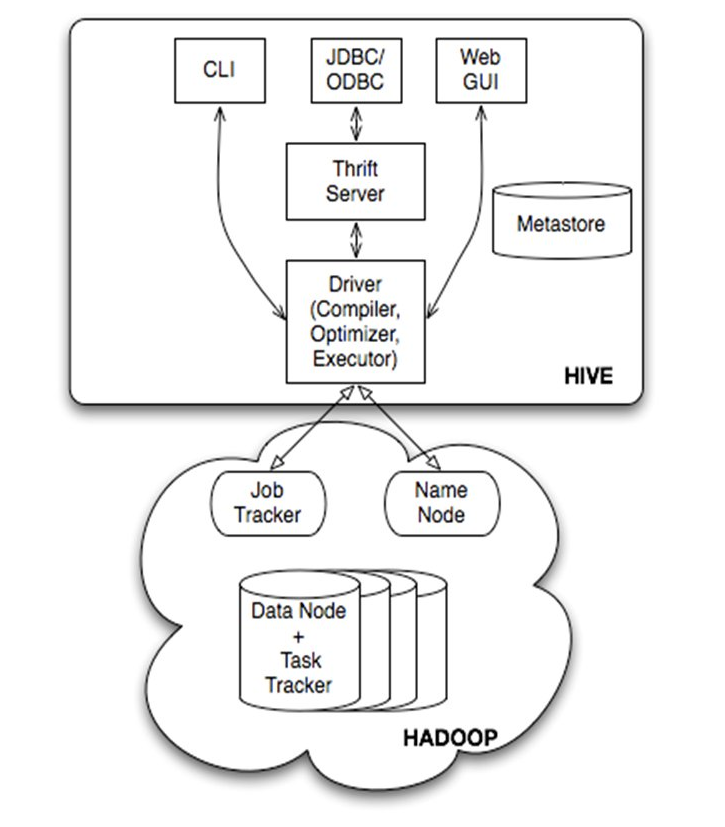
\includegraphics[width=.6\linewidth]{figures/hive.png}
\caption{hive基础架构图}\label{fig-hive-1}
\end{figure} 
\par \textbf{Driver}组件:该组件包括Complier、Optimizer和Executor,它的作用是将我们写的HiveQL(类SQL)语句进行解析、编译优化,生成执行计划,然后调用底层的mapreduce计算框架。
\par \textbf{Metastore}组件:元数据服务组件,这个组件存储hive的元数据,hive的元数据存储在关系数据库里,hive支持的关系数据库有derby、mysql。元数据对于hive十分重要,因此hive支持把metastore服务独立出来,安装到远程的服务器集群里,从而解耦hive服务和metastore服务,保证hive运行的健壮性。
\par \textbf{Thrift}服务:thrift是facebook开发的一个软件框架,它用来进行可扩展且跨语言的服务的开发,hive集成了该服务,能让不同的编程语言调用hive的接口。
客户端组件:
\par \textbf{CLI}:command line interface,命令行接口。
\par \textbf{Thrift客户端}:上面的架构图里没有写上Thrift客户端,但是hive架构的许多客户端接口是建立在thrift客户端之上,包括JDBC和ODBC接口。
\par \textbf{WEBGUI}:hive客户端提供了一种通过网页的方式访问hive所提供的服务。这个接口对应hive的hwi组件(hive web interface),使用前要启动hwi服务。
\par Hive的metastore组件是hive元数据集中存放地。Metastore组件包括两个部分:metastore服务和后台数据的存储。后台数据存储的介质就是关系数据库,例如hive默认的嵌入式磁盘数据库derby,还有mysql数据库。Metastore服务是建立在后台数据存储介质之上,并且可以和hive服务进行交互的服务组件,默认情况下,metastore服务和hive服务是安装在一起的,运行在同一个进程当中。也可以把metastore服务从hive服务里剥离出来,metastore独立安装在一个集群里,hive远程调用metastore服务,这样可以把元数据这一层放到防火墙之后,客户端访问hive服务,就可以连接到元数据这一层,从而提供了更好的管理性和安全保障。使用远程的metastore服务,可以让metastore服务和hive服务运行在不同的进程里,这样也保证了hive的稳定性,提升了hive服务的效率。
\begin{figure}[htbp]
\centering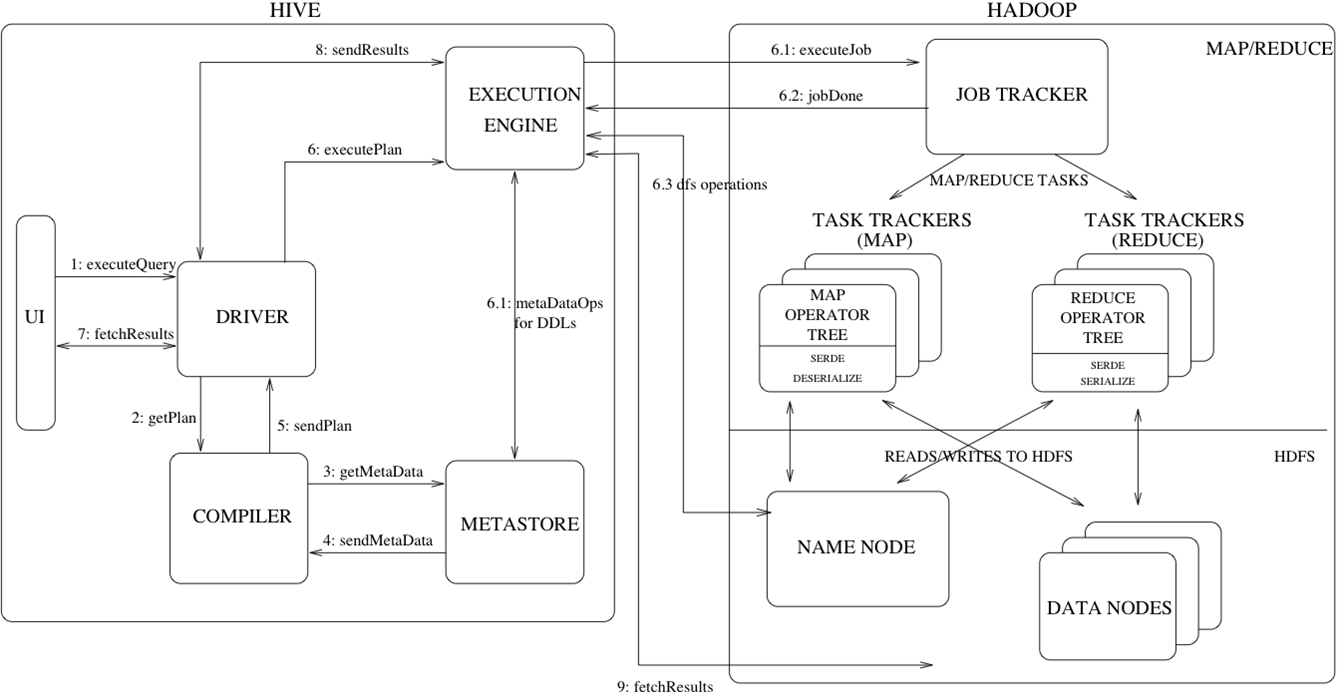
\includegraphics[width=\linewidth]{figures/hive-2.png}
\caption{hive执行流程}\label{fig-hive-2}
\end{figure} 
\subsection{hive与关系数据库的区别}
\par 关系数据库里,表的加载模式是在数据加载时候强制确定的(表的加载模式是指数据库存储数据的文件格式),如果加载数据时候发现加载的数据不符合模式,关系数据库则会拒绝加载数据,这个就叫“写时模式”,写时模式会在数据加载时候对数据模式进行检查校验的操作。Hive在加载数据时候和关系数据库不同,hive在加载数据时候不会对数据进行检查,也不会更改被加载的数据文件,而检查数据格式的操作是在查询操作时候执行,这种模式叫“读时模式”。在实际应用中,写时模式在加载数据时候会对列进行索引,对数据进行压缩,因此加载数据的速度很慢,但是当数据加载好了,我们去查询数据的时候,速度很快。但是当我们的数据是非结构化,存储模式也是未知时候,关系数据操作这种场景就麻烦多了,这时候hive就会发挥它的优势。
\par 关系数据库一个重要的特点是可以对某一行或某些行的数据进行更新、删除操作,hive不支持对某个具体行的操作,hive对数据的操作只支持覆盖原数据和追加数据。Hive也不支持事务和索引。更新、事务和索引都是关系数据库的特征,这些hive都不支持,也不打算支持,原因是hive的设计是海量数据进行处理,全数据的扫描是它的工作常态,针对某些具体数据进行操作的效率是很差的,对于数据的添加操作,hive是通过查询将原表的数据进行转化最后存储在新表里,这和传统数据库的更新操作有很大不同。
\par Hive也可以在hadoop做实时查询上做一份自己的贡献,那就是和hbase集成,hbase可以进行快速查询,但是hbase不支持类SQL的语句,那么此时hive可以给hbase提供sql语法解析的外壳,可以用类sql语句操作hbase数据库。今天的hive就写到这里,关于hive我打算一共写三篇文章,这是第一篇,下一篇主要讲hive支持的数据模型,例如:数据库(database)、表(table)、分区(partition)和桶(bucket),还有hive文件存储的格式,还有hive支持的数据类型。第三篇文章就会讲到hiveQL的使用、以及结合mapreduce查询优化的技术和自定义函数,以及我们现在在公司项目里运用hive的实例。马云在退休的时候说互联网现在进入了大数据时代,大数据是现在互联网的趋势,而hadoop就是大数据时代里的核心技术,但是hadoop和mapreduce操作专业型太强,所以facebook在这些的基础上开发了hive框架,毕竟世界上会sql的人比会java的人多的多,hive是可以说是学习hadoop相关技术的一个突破口,哪些自立于投身hadoop技术开发的童鞋们,可以先从hive开始哦。
\subsection{hive的join类型简介}
\par 作为数据分析中经常进行的join操作,传统DBMS数据库已经将各种算法优化到了极致,而对于hadoop使用的mapreduce所进行的join操作,去年开始也是有各种不同的算法论文出现,讨论各种算法的适用场景和取舍条件,本文讨论hive中出现的几种join优化,然后讨论其他算法实现,希望能给使用hadoop做数据分析的开发人员提供一点帮助。
\par Facebook今年在yahoo的hadoop summit大会上做了一个关于最近两个版本的hive上所做的一些join的优化,其中主要涉及到hive的几个关键特性:值分区,hash分区,map join,index。
\subsubsection{Common Join}
\par 最为普通的join策略,不受数据量的大小影响,也可以叫做reduce side join,最没效率的一种join方式. 它由一个mapreduce job完成.首先将大表和小表分别进行map操作,在map shuffle的阶段每一个\textbf{map output key}变成了\textbf{table-name-tag-prefix + join-column-value}, 但是在进行partition的时候它仍然只使用\textbf{join-column-value}进行hash.
\par 每一个reduce接受所有的map传过来的split,在reducce的shuffle阶段,它将\textbf{map output key}前面的\textbf{table-name-tag-prefix}给舍弃掉进行比较. 因为reduce的个数可以由小表的大小进行决定,所以对于每一个节点的reduce一定可以将小表的split放入内存变成hashtable,然后将大表的每一条记录进行一条一条的比较.
\subsubsection{Map Join}
\par Map Join的计算步骤分两步,将小表的数据变成hashtable,广播到所有的map端,将大表的数据进行合理的切分,然后在map阶段的时候用大表的数据一行一行的去探测(probe)小表的hashtable.如果join key相等,就写入HDFS.Map Join之所以叫做Map Join是因为它所有的工作都在map端进行计算.
\par hive在Map Join上做了几个优化:hive 0.6的时候默认认为写在select后面的是大表,前面的是小表,或者使用\textbf{+mapjoin(map\_table)}提示进行设定.hive 0.7的时候这个计算是自动化的,它首先会自动判断哪个是小表,哪个是大表,这个参数由\textbf{(hive.auto.convert.join=true)}来控制。小表的大小由\textbf{(hive.smalltable.filesize)}参数控制(默认是25M),当小表超过这个大小,hive会默认转化成Common Join。
\par 首先小表的Map阶段它会将自己转化成MapReduce Local Task,然后从HDFS上取小表的所有数据,将自己转化成Hashtable file并压缩打包放入DistributedCache里面.
\par 目前hive的map join有几个限制,一个是它打算用BloomFilter来实现hashtable,BloomFilter大概比hashtable省8-10倍的内存, 但是BloomFilter的大小比较难控制.现在DistributedCache里面hashtable默认的复制是3份,对于一个有1000个map的大表来说,这个数字太小,大多数map操作都等着DistributedCache复制.
\subsubsection{Bucket Map Join}
\par hive建表的时候支持hash分区通过指定clustered by(col\_name,xxx) into number\_buckets,当连接的两个表的join key就是bucket column的时候,就可以通过\textbf{hive.optimize.bucketmapjoin=true}来控制hive执行\textbf{bucket map join}了, 需要注意的是小表的number\_buckets必须是大表的倍数.无论多少个表进行连接这个条件都必须满足。(其实如果都按照2的指数倍来分bucket, 大表也可以是小表的倍数,不过这中间需要多计算一次,对int有效,long和string不清楚)。
\par \textbf{Bucket Map Join}执行计划分两步,第一步先将小表做map操作变成hashtable,然后广播到所有大表的map端,大表的map端接受了number\_buckets个小表的hashtable并不需要合成一个大的hashtable,直接可以进行map操作,map操作会产生number\_buckets个split,每个split的标记跟小表的hashtable标记是一样的, 在执行projection操作的时候,只需要将小表的一个hashtable放入内存即可,然后将大表的对应的split拿出来进行判断,所以其内存限制为小表中最大的那个hashtable的大小.
\par \textbf{Bucket Map Join}同时也是\textbf{Map Side Join}的一种实现,所有计算都在Map端完成,没有Reduce的都被叫做\textbf{Map Side Join},\textbf{Bucket只是hive的一种hash partition的实现},\textbf{另外一种当然是值分区:create table a  (xxx) partition by (col\_name)}
\par 一般hive中两个表不一定会有同一个partition key, 即使有也不一定会是join key.所以hive没有这种基于值的map side join,hive中的list partition主要是用来过滤数据的而不是分区.两个主要参数为(hive.optimize.cp = true 和hive.optimize.pruner=true).
\par hadoop源代码中默认提供\textbf{Map Side Join}的实现,可以在hadoop源码的src/contrib/data\_join/src目录下找到相关的几个类.其中TaggedMapOutput即可以用来实现hash也可以实现list,看你自己决定怎么分区. Hadoop Definitive Guide第8章关于\textbf{Map Side Join}和\textbf{side data distribution}章节也有一个例子示例怎样实现值分区的map side join.
\subsubsection{Where条件查询}
\par 当使用hive进行where查询时,例如\textsl{'select * from cable.testData where cardId=80000364;'}由于hive默认的,每个MapTask的输入块大小为256MB,因此对14664.9MB的文件,大概需要57个MapTask,由于where条件查询,不需要进行reduce运算,因此ReduceTask数目为0,此时可以通过设置\textsl{set mapred.max.split.size=128000000;},对上述例子,可生成112个MapTask。在两亿多条记录中(共2,3235,9109条记录)查询,耗费时间67S(57个MapTask时,112个MapTask耗费时间约79S)。
% \par \textbf{Bucket Map Join}并没有解决map join在小表必须完全装载进内存的限制, 如果想要在一个reduce节点的大表和小表都不用装载进内存,必须使两个表都在join key上有序才行,你可以在建表的时候就指定\textbf{sorted by join key}或者使用index的方式.
% \begin{verbatim}
% set hive.optimize.bucketmapjoin = true;
% set hive.optimize.bucketmapjoin.sortedmerge = true;
% set hive.input.format=org.apache.hadoop.hive.ql.io.BucketizedHiveInputFormat;
% Bucket columns == Join columns == sort columns
% \end{verbatim}
% \par 这样小表的数据可以每次只读取一部分,然后还是用大表一行一行的去匹配,这样的join没有限制内存大小,并且也可以执行全外连接.
% \par 真实数据中数据倾斜是一定的, hadoop中默认是使用hive.exec.reducers.bytes.per.reducer = 1000000000,也就是每个节点的reduce默认是处理1G大小的数据,如果你的join操作也产生了数据倾斜,那么你可以在hive中设定
% \begin{verbatim}
% set hive.optimize.skewjoin = true; 
% set hive.skewjoin.key = skew_key_threshold(default=100000)
% \end{verbatim}
% \par hive在运行的时候没有办法判断哪个key会产生多大的倾斜,所以使用这个参数控制倾斜的阈值,如果超过这个值,新的值会发送给那些还没有达到的reduce, 一般可以设置成(处理的总记录数/reduce个数)的2-4倍都可以接受.倾斜是经常存在的,一般select的层数超过2层,翻译成执行计划多于3个以上的mapreduce job都很容易产生倾斜,建议每次运行比较复杂的sql之前都可以设一下这个参数.如果你不知道设置多少,可以就按官方默认的1个reduce只处理1G的算法,那么skew\_key\_threshold= 1G/平均行长. 或者默认直接设成250000000 (差不多算平均行长4个字节).
% \par hive中没有in/exist这样的子句,所以需要将这种类型的子句转成\textbf{Left Semi Join}.\textbf{Left Semi Join}是只传递表的join key给map阶段,如果key足够小还是执行map join, 如果不是则还是common join.Join策略中的难点:大多数只适合等值连接(equal join),范围比较和全外连接没有合适的支持,提前分区,临时分区,排序,多种不同执行计划很难评价最优方案。没有考虑IO,比如临时表,网络消耗和网络延迟时间,CPU时间,最优的方案不代表系统资源消耗最少。
\subsection{Hive提供的索引功能}
\par Hive提供有限的索引功能,这不像传统的关系型数据库那样有“键(key)”的概念,用户可以在某些列上创建索引来加速某些操作,给一个表创建的索引数据被保存在另外的表中。Hive的索引功能现在还相对较晚,提供的选项还较少。但是,索引被设计为可使用内置的可插拔的java代码来定制,用户可以扩展这个功能来满足自己的需求。
\par 当然不是所有的查询都会受惠于Hive索引。用户可以使用EXPLAIN语法来分析HiveQL语句是否可以使用索引来提升用户查询的性能。像RDBMS中的索引一样,需要评估索引创建的是否合理,毕竟,索引需要更多的hdfs磁盘空间,并且创建维护索引也会有一定的代价。用户必须要权衡从索引得到的好处和代价。先建立一个临时表,避免覆盖我精心准备的表,\textsl{create table cable.TempTable as select cardId,Date,Time as text from cable.testData;}在TempTable的cardId列上,建立索引,耗费时间:200.727S,下面在cardId列上建立一个索引:
\begin{verbatim}
create index TempTable_index on table TempTable(cardId)
as 'org.apache.hadoop.hive.ql.index.compact.CompactIndexHandler'
with deferred rebuild;
alter index TempTable_index on TempTable rebuild;
--现在建立了索引表TempTable_index
--通过下述命令,可以查询TempTable_index内容
select * from cable.cable__temptable_temptable_index__ limit 10;
-- 下面是使用索引的过程,/tmp/table02_index_data为hdfs上目录;
Insert overwrite directory "/tmp/table02_index_data" 
select `_bucketname`,`_offsets` from cable.cable__temptable_temptable_index__ 
where cardId = 80000000;
Set hive.index.compact.file=/tmp/table02_index_data;
Set hive.optimize.index.filter=false;
Set hive.input.format = 
org.apache.hadoop.hive.ql.index.compact.HiveCompactIndexInputFormat;
select * from cable.TempTable where cardId=80000000;
\end{verbatim}
\par 使用后,查询耗时约13.246S,而不使用索引时,耗时约61.907S,但执行\textsl{select `\_bucketname`,`\_offsets` from cable.cable\_\_temptable\_temptable\_index\_\_ where id = 80000000;}这一步耗时约51.635S,总体上得不偿失。
在本示例中,在employees上创建了名为employees\_index的索引,索引数据存放在employees\_index\_table索引表中,WITH DEFERRED REBUILD表明创建一个空索引,可以在之后使用如下语句创建索引数据:
\begin{verbatim}
ALTER INDEX employees_index ON TABLE employees 
PARTITION(country = 'US') REBUILD;
\end{verbatim}
\par PARTITIONED BY表明只对某个分区创建索引,若没有该选项则表示对所有分区都创建索引,另外要注意的是index的分区索引默认是和表的分区一致的,也不能对视图VIEW创建索引。
AS 'org.apache.hadoop.hive.ql.index.compact.CompactIndexHandler'表示使用Apache的org.apache.hadoop.hive.ql.index.compact.CompactIndexHandler作为创建索引的handler,当然也可以使用第三方的实现类或其他的实现类。当然也可以对其他字段创建索引。 
\par Bitmap位图索引:Hive v0.80添加了一个内置的bitmap位图索引。Bitmap位图索引通常适用于只有少数不同值的列。现在我们修改上一个索引示例为位图索引:
\begin{verbatim}
CREATE INDEX employees_index
ON TABLE employees (country)
AS 'BITMAP'
WITH DEFERRED REBUILD
IDXPROPERTIES ('creator' = 'me','created_at' = 'some_time')
IN TABLE employees_index_table
PARTITIONED BY (country,name)
COMMENT 'Employees indexed by country and name.';
\end{verbatim}
重建索引:如果用户在创建索引时指定WITH DEFERRED REBUILD关键字,那么开始时是一个空索引。我们在任何时候使用ALTER INDEX语句来创建或重建索引:
\begin{verbatim}
ALTER INDEX employees_index ON TABLE employees 
PARTITION(country = 'US')
REBUILD;
\end{verbatim}
\par Hive没有提供一个内置的在数据变更时自动触发创建索引的机制,故用户需要自己通过ALTER INDEX语句来创建索引;另外,重建索引操作是一个原子操作,因此当rebuild失败时,已构建的索引也无法使用。
查看索引:用户可以查看某个表上的所有的索引:
\begin{verbatim}
SHOW FORMATTED INDEX ON employees;
SHOW FORMATTED INDEXES ON employees;
\end{verbatim}
删除索引:在删除一个索引的时候,也会同时删除索引数据所在的表,如:
\begin{verbatim}
DROP INDEX IF EXISTS employees_index ON TABLE employees;
\end{verbatim}





